\documentclass{standalone}
\usepackage{tikz}
\usetikzlibrary{chains, fit}

\begin{document}
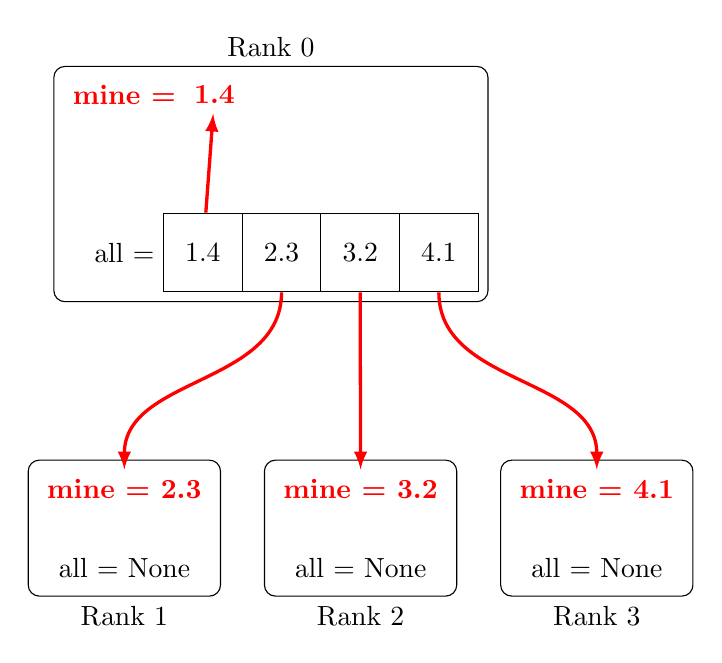
\begin{tikzpicture}
\tikzset{
  arrow/.style={
    >=latex
  },
  line/.style={
    draw,
    ->,
    very thick,
  },
  array/.style={
    draw,
    minimum size=1cm
  },
  new/.style={
    red,
    font=\bfseries
  },
  old/.style={
  }
}

% Initialize
%\newcommand{\allzero}{1.4}
%\newcommand{\allone}{2.3}
%\newcommand{\alltwo}{3.2}
%\newcommand{\allthree}{4.1}
%\newcommand{\minezero}{0}
%\newcommand{\mineone}{0}
%\newcommand{\minetwo}{0}
%\newcommand{\minethree}{0}
%\newcommand{\allstyle}{new}
%\newcommand{\minestyle}{old}
%\newcommand{\drawarrows}{}

% Scatter
\newcommand{\allzero}{1.4}
\newcommand{\allone}{2.3}
\newcommand{\alltwo}{3.2}
\newcommand{\allthree}{4.1}
\newcommand{\minezero}{\allzero}
\newcommand{\mineone}{\allone}
\newcommand{\minetwo}{\alltwo}
\newcommand{\minethree}{\allthree}
\newcommand{\allstyle}{old}
\newcommand{\minestyle}{new}
\newcommand{\drawarrows}{
  \draw[red, line, arrow] (all00) to (mine0);
  \draw[red, line, arrow, out=270, in=90] (all01) to (mine1);
  \draw[red, line, arrow, out=270, in=90] (all02) to (mine2);
  \draw[red, line, arrow, out=270, in=90] (all03) to (mine3);
}

% Compute
%\newcommand{\allzero}{1.4}
%\newcommand{\allone}{2.3}
%\newcommand{\alltwo}{3.2}
%\newcommand{\allthree}{4.1}
%\newcommand{\minezero}{15.4}
%\newcommand{\mineone}{25.3}
%\newcommand{\minetwo}{35.2}
%\newcommand{\minethree}{45.1}
%\newcommand{\allstyle}{old}
%\newcommand{\minestyle}{new}
%\newcommand{\drawarrows}{}

% Gather
%\newcommand{\minezero}{15.4}
%\newcommand{\mineone}{25.3}
%\newcommand{\minetwo}{35.2}
%\newcommand{\minethree}{45.1}
%\newcommand{\allzero}{\minezero}
%\newcommand{\allone}{\mineone}
%\newcommand{\alltwo}{\minetwo}
%\newcommand{\allthree}{\minethree}
%\newcommand{\allstyle}{new}
%\newcommand{\minestyle}{old}
%\newcommand{\drawarrows}{
%  \draw[red, line, arrow] (mine0) to (all00);
%  \draw[red, line, arrow, out=90, in=270] (mine1) to (all01);
%  \draw[red, line, arrow, out=90, in=270] (mine2) to (all02);
%  \draw[red, line, arrow, out=90, in=270] (mine3) to (all03);
%}

% Rank 0
\begin{scope}[
  start chain=1 going right, node distance=-0.15 mm
  ]
\node (all0start) [on chain=1, draw=none, \allstyle] {all = };
\node (all00) [on chain=1, array, \allstyle] {\allzero};
\node (all01) [on chain=1, array, \allstyle] {\allone};
\node (all02) [on chain=1, array, \allstyle] {\alltwo};
\node (all03) [on chain=1, array, \allstyle] {\allthree};
\end{scope}

\begin{scope}[
  shift={(0,2cm)},
  start chain=2 going right, node distance=-0.15 mm
  ]
\node (mine0start) [on chain=2, \minestyle] {mine =};
\node (mine0) [on chain=2, \minestyle] {\minezero};
\end{scope}

\node (rank0) [fit=(all00) (all01) (all02) (all03) (all0start) (mine0start) (mine0), label=above:{Rank 0}, draw, rounded corners] {};

% Rank 1
\begin{scope}[
  shift={(-0cm, -4cm)},
  start chain=3 going right, node distance=-0.15 mm
  ]
\node (all1start) [on chain=3, draw=none] {all = None};
\end{scope}

\begin{scope}[
  shift={(-0cm,-3cm)},
  start chain=4 going right, node distance=-0.15 mm
  ]
\node (mine1) [on chain=4, \minestyle] {mine = \mineone};
\end{scope}

\node (rank1) [fit=(all1start) (mine1), label=below:{Rank 1}, draw, rounded corners] {};

% Rank 2
\begin{scope}[
  shift={(3cm, -4cm)},
  start chain=5 going right, node distance=-0.15 mm
  ]
\node (all2start) [on chain=5, draw=none] {all = None};
\end{scope}

\begin{scope}[
  shift={(3cm,-3cm)},
  start chain=6 going right, node distance=-0.15 mm
  ]
\node (mine2) [on chain=6, \minestyle] {mine = \minetwo};
\end{scope}

\node (rank2) [fit=(all2start) (mine2), label=below:{Rank 2}, draw, rounded corners] {};

% Rank 3
\begin{scope}[
  shift={(6cm, -4cm)},
  start chain=7 going right, node distance=-0.15 mm
  ]
\node (all3start) [on chain=7, draw=none] {all = None};
\end{scope}

\begin{scope}[
  shift={(6cm,-3cm)},
  start chain=8 going right, node distance=-0.15 mm
  ]
\node (mine3) [on chain=8, \minestyle] {mine = \minethree};
\end{scope}

\node (rank3) [fit=(all3start) (mine3), label=below:{Rank 3}, draw, rounded corners] {};

\drawarrows

\end{tikzpicture}

\end{document}
